\section{Técnicas para la Evaluación de Modelos Predictivos}

%En este punto, se puede hablar de conjunto de test, train etc TO DO

El estudio que se realiza en esta sección es sobre modelos predictivos de clasificación, el objetivo de un modelo de clasificación es predecir la clase de un registro en base al resto de atributos. Los modelos de clasificación binaria, son modelos predictivos en los que el hay dos clases, de forma genérica se definen las dos clases como clase Positiva y clase Negativa. Los modelos de clasificación multi etiqueta se definen como modelos de clasificación con mas de dos clases. La evaluación del modelo corresponde con una de las últimas fases del proceso de predictivo, en esta fase se necesita un conjunto de datos en el que por cada registro se tenga la clase real y la clase que predice el modelo.

\bigbreak

En esta sección se propone una revisión de los principales métodos para la evaluación de modelos predictivos. El objetivo principal es introducir cada un de los métodos, también se incluye un análisis de cada método en que se trata cuando aplicar el método, la interpretación de los resultados, si el método solo es valido para modelos de clasificación binaria, si es sensible al balance entre el número de instancias de cada clases, etc.

\subsection{Matriz de confusión}

La matriz de confusión es una herramienta que se suele aplicar en las primeras fases del análisis, permite organizar los indicadores de rendimiento obtenidos para un modelo predictivo, en general, ofrece un recuento de los registros en base a la clase real de cada registro y a la predicción que realiza el modelo. La matriz de confusión se define como una matriz cuadrada de $NxN$ elementos donde $N$ es el número de clases del modelo, en cada fila de la matriz se define la clase real del registro y en cada columna se define la clase predicha por el modelo o viceversa.

\bigbreak

En la matriz de confusión se definen cuatro indicadores, estos indicadores ofrecen una visión general del rendimiento del modelo y son la base para el cálculo de algunos métodos más avanzados que se tratan en secciones posteriores de este documento. Los indicadores definidos en la matriz de confusión son:

\begin{itemize}
    \item Verdadero Positivo: Registros de clase real positiva y en los que la predicción se hace correctamente.
    \item Verdadero Negativo: Registros de clase real negativa y en los que la predicción se hace correctamente.
    \item Falso Negativo: Registros de clase real positiva y en los que la predicción se hace incorrectamente.
    \item Falso Positivo: Registros de clase real negativa y en los que la predicción se hace incorrectamente.
\end{itemize}

La matriz de confusión se define de forma general para modelos de clasificación multi etiqueta, sin embargo, a la hora de obtener los indicadores de rendimiento para modelos de clasificación con más de dos clases tenemos que definir $N$ matrices una por cada clase del modelo. En cada matriz se define positiva una de las clases y se agrupan como negativas el resto, de esta forma, el estudio que se realiza a partir de las diferentes sub matrices ya no es un estudio global, sino que es específico para cada clase concreta.

\begin{table}[htp]
    \small
    \centering
    \begin{tabularx}{150pt}{Y Y Y}
            & P$^{\prime}$  & N$^{\prime}$    \\\hline
        P   & TP            & FN              \\\hline
        N   & FP            & TN              \\\hline
    \end{tabularx}

    \caption{Matriz de confusión 2x2. Las etiquetas P$^{\prime}$ y N$^{\prime}$ hacen referencia a registros que se predicen positivos y negativos respectivamente. Esta nomenclatura se utiliza a lo largo del documento en más ocasiones.}
    \label{tab:1}
\end{table}

%%%%%%%%%%%%%%%%%%%%%%%%%%%%%%%%%%%%%%%%%%%%%%%%%%%%%%%%% SUBSECCION METODOS ESTADISTICOS

\subsection{Métodos Analíticos}

%%%%%%%%%%%%%%%%%%%%%%%%%%%%% SUBSUBSECCION Exactitud

\subsubsection{Exactitud}

La exactitud \cite{tharwat_2018} es una de las medidas más utilizadas a la hora de establecer la calidad general de un modelo predictivo, se define como un indicador que representa la tasa de acierto del modelo sobre instancias positivas y negativas. El cálculo de esta medida se hace en base a los cuatro indicadores de rendimiento definidos en la matriz de confusión. Hay que tener en cuenta que la exactitud es un método sensible a grandes diferencias entre el numero de instancias positivas y negativas, en la ecuación \ref{eq:ACC_BAL} se puede comprobar que al variar el valor de $\alpha$ la igualdad no se mantiene. El resultado que se obtiene al aplicar el método se encuentra en el intervalo de cero a uno, los valores próximos a cero corresponden a modelos con una baja tasa de acierto, mientras que los valores próximos a uno indican una alta tasa de acierto. En términos generales, los modelos que obtienen un resultado inferior a media unidad son poco prometedores, en promedio tienen una tasa de acierto inferior a la de un modelo de clasificación aleatoria. Por último, cabe destacar que la exactitud es un método independiente del número de clases, se puede aplicar tanto a modelos de clasificación binaria como a modelos de clasificación multi etiqueta.

\bigbreak

\begin{equation}
    ACC = \frac{TP+TN}{TP+TN+FP+FN}
    \label{eq:ACC}  
\end{equation}

\bigbreak

\begin{equation}
    \frac{TP+TN}{TP+TN+FP+FN}\neq \frac{ \alpha \cdot TP+TN}{\alpha \cdot TP+TN+FP+ \alpha \cdot FN}
    \label{eq:ACC_BAL}  
\end{equation}


%%%%%%%%%%%%%%%%%%%%%%%%%%%%% SUBSUBSECCION SENSIBILIDAD Y ESPECIFICIDAD

\subsubsection{Sensibilidad y Especificidad}

La sensibilidad y la especificidad \cite{Florkowski2008}\cite{tharwat_2018} son dos métodos complementarios que ofrecen una representación de la exactitud del modelo separando los registros en base a la clase. La sensibilidad es un método que mide la tasa de acierto del modelo sobre instancias de clase positiva. De igual forma, la especificidad mide la tasa de acierto del modelo sobre instancias de clase negativa. La separación que se establece en base a la clase implica que tanto la sensibilidad como la especificidad se pueden aplicar de forma independiente a la variación del número de instancias de cada clase. En ambos casos el cálculo se hace a partir de los indicadores de rendimiento definidos en la matriz de confusión. El resultado obtenido se encuentra en el intervalo de cero a uno, los valores próximos a cero indican una baja tasa de acierto, mientras que los valores próximos a uno indican una alta tasa de acierto. A diferencia de la exactitud estos dos métodos son sensibles al número de clases del modelo, están diseñados para su aplicación únicamente a modelos de clasificación binaria.

\bigbreak

\begin{equation}
    TPR = \frac{TP}{P} = \frac{TP}{TP+FN}
    \label{eq:TPR}      
\end{equation}

\bigbreak

\begin{equation}
    TNR = \frac{TN}{N} = \frac{TN}{TN+FP}
    \label{eq:TNR}    
\end{equation}

%%%%%%%%%%%%%%%%%%%%%%%%%%%%% SUBSUBSECCION PRECISION Y PRECISION INVERSA

\subsubsection{Precisión y Precisión Inversa}

La precisión y la precisión inversa \cite{tharwat_2018} son métodos que miden la exactitud del modelo en base a la predicción que realiza. La precisión es un método que mide la tasa de acierto del modelo sobre instancias que se predicen positivas. De la misma forma, la precisión inversa se define como la tasa de aciertos del modelo sobre instancias que se predicen negativas. Los métodos se ven afectados al aumentar considerablemente el numero de instancias de una determinada clase. El cálculo se hace a partir de los indicadores de rendimiento definidos en la matriz de confusión, en ambos casos el resultado obtenido indica mejores tasas de acierto cuanto mas se aproxime a la unidad. Los métodos son sensibles al número de clases que se definen en el modelo, su aplicación es exclusiva para modelos de clasificación binaria.

\bigbreak

\begin{equation}
    PPV = \frac{TP}{P^{\prime}} = \frac{TP}{TP+FP}
    \label{eq:PPV}
\end{equation}

\bigbreak

\begin{equation}
    NPV = \frac{TN}{N^{\prime}} = \frac{TN}{TN+FN}
    \label{eq:NPV}
\end{equation}

%%%%%%%%%%%%%%%%%%%%%%%%%%%%% SUBSUBSECCION RAZON DE VEROSIMILITUD

\subsubsection{Razones de Verosimilitud}

Las razones de verosimilitud son métodos que se utilizan fundamentalmente en el ámbito médico para la evaluación de pruebas diagnósticas. Los indicadores miden como varia la probabilidad de padecer una determinada patología en función de si el paciente presenta o no presenta un estado concreto. De forma similar, para el ámbito de la evaluación de modelos predictivos las razones de verosimilitud nos informan de cómo varia la probabilidad de que un registro sea positivo en función de la predicción que realiza el modelo.

\bigbreak

Tenemos dos tipos de razones de verosimilitud, la razón de verosimilitud positiva LR+ y la razón de verosimilitud negativa LR-. La razón de verosimilitud positiva mide como varia la probabilidad de que un registro sea positivo cuando se clasifica como positivo. Por otro lado, la razón de verosimilitud negativa mide como varia la probabilidad de que un registro sea positivo cuando se clasifica como negativo. En ambos casos el cálculo de los métodos se hace a partir de la sensibilidad y la especificidad. Es importante destacar que las razones de verosimilitud no guardan una relación de proporcionalidad, el cambio en la probabilidad de que un registro sea de clase positiva no varía en la misma proporción cuando el registro se clasifica como positivo que cuando se clasifica como negativo.

\bigbreak

\begin{equation}
    LR^{\phantom{.}+}    = \frac{TPR}{1-TNR}
    \label{eq:LR+}   
\end{equation}

\bigbreak

\begin{equation}
    LR^{\phantom{.}-} = \frac{1-TPR}{TNR}
    \label{eq:LR-}
\end{equation}

\bigbreak

La razón de verosimilitud positiva es una medida que toma valores mayores que la unidad, ofrece un mejor indicador cuanto mayor sea el valor que toma. Por el contrario, la razón de verosimilitud negativa se encuentra en el rango de valores de cero a uno, ofrece un mejor indicador cuanto más próximo al cero se encuentre. En ambos casos los valores próximos a la unidad indican que el modelo no tiene capacidad discriminatoria, es decir, la predicción que se realiza no varía la probabilidad de pertenecer a la clase positiva. En la Tabla \ref{tab:2} podemos ver una aproximación de la variación en la probabilidad de pertenecer a la clase positiva para diferentes razones de verosimilitud.

\bigbreak

\begin{table}[htp]
    \small
    \centering
    \begin{tabular}{l l l}
        Variación (\%) & \hspace{10pt}LR+ & \hspace{10pt}LR- \\\hline
        +45            & \hspace{10pt}10  & \hspace{10pt}-   \\\hline
        +30            & \hspace{10pt}5   & \hspace{10pt}-   \\\hline
        +15            & \hspace{10pt}2   & \hspace{10pt}-   \\\hline
        0              & \hspace{10pt}1   & \hspace{10pt}1   \\\hline
        -15            & \hspace{10pt}-   & \hspace{10pt}0.5 \\\hline
        -30            & \hspace{10pt}-   & \hspace{10pt}0.2 \\\hline
        -45            & \hspace{10pt}-   & \hspace{10pt}0.1 \\\hline
    \end{tabular}

    \caption{Variación en la probabilidad de pertenecer a la clase positiva para diferentes razones de verosimilitud \cite{McGee2002}.}
    \label{tab:2}
\end{table}

\bigbreak
%% CAMBIAR NORMAL POR TUMORAL

%En la Tabla \ref{tab:3} tenemos los resultados obtenidos para el fichero de datos breast\_gse26910.csv incluido en el apartado de experimentación. La clase Normal presenta un LR+ de 4 unidades, esto implica un aumento moderado (entre un 15\% y un 30\%) de la probabilidad que tiene un registro de pertenecer a la clase Normal cuando el modelo predice Normal el registro. Por otro lado, la clase Normal presenta un LR- de 0.4 unidades esto supone de nuevo una disminución moderada (entre un 15\% y un 30\%) de la probabilidad que tiene un registro de pertenecer a la clase Normal cuando el modelo predice Tumoral el registro.

%%%%%%%%%%%%%%%%%%%%%%%%%%%%% SUBSUBSECCION DOR

\subsubsection{Diagnostic Odds Ratio}

El DOR \cite{dor_2003} es un método que surge a partir de la necesidad de tener un solo indicador de rendimiento que sea fácil de interpretar. Este método no depende del balance entre el número de registros positivos y negativos, en otros métodos como por ejemplo la exactitud esta cuestión presenta un problema la hora de obtener resultados concluyentes. El DOR se calcula a partir de las razones de verosimilitud, se define como el cociente de la razón de verosimilitud positiva entre la razón de verosimilitud negativa. El resultado que ofrece es un valor mayor que cero, cuanto mayor sea este valor mejor rendimiento presentará el modelo.

\bigbreak

\begin{equation}
    DOR = \frac{LR^{\phantom{.}+}}{LR^{\phantom{.}-}} = \frac{TPR}{1-TNR} \cdot \frac{TNR}{1-TPR} = \frac{TP \cdot TN}{FP \cdot FN}
    \label{eq:DOR}
\end{equation}

\bigbreak

%En la Tabla \ref{tab:4} tenemos los resultados obtenidos para el fichero de datos breast\_gse26910.csv incluido en el apartado de experimentación. La clase Tumoral presenta un DOR de 10 unidades, esto implica que para un registro que se predice Tumoral la probabilidad de ser Tumoral es 10 veces mayor que la de ser Normal.

%%%%%%%%%%%%%%%%%%%%%%%%%%%%% SUBSUBSECCION ÍNDICE YOUDEN

\subsubsection{Índice Youden}

El índice de Youden \cite{Youden1950} se define como la suma de la sensibilidad y la especificidad menos la unidad, ofrece un indicador de rendimiento independiente de la diferencia entre el número de registros de cada clase. El resultado que ofrece se encuentra en el intervalo $[-1, 1]$, los valores próximos a -1 indican una casi nula capacidad discriminatoria entre clases, por otro lado, un resultado próximo a 1 indica una alta capacidad discriminatoria. El índice Youden pondera de la misma forma la sensibilidad que la especificidad, para un modelo balanceado que clasifica positivos todos los registros tendrá un resultado de 0 lo que se puede interpretar como un modelo poco prometedor. Para obtener un resultado que este próximo a la unidad es necesario que el modelo tenga buenas tasas de sensibilidad y especificidad, en general el índice Youden penaliza resultados bajos de sensibilidad y/o especificidad.
\bigbreak

\begin{equation}
    YI = TPR + TNR - 1
    \label{eq:YI}
\end{equation}

\bigbreak

%En la Tabla \ref{tab:5} tenemos los resultados obtenidos para el fichero de datos breast\_gse26910.csv incluido en el apartado de experimentación. Este caso práctico muestra un índice de Youden de 0.5 esto implica que la predicción que hace el modelo tiene una capacidad discriminatoria entre clases aceptable.


%%%%%%%%%%%%%%%%%%%%%%%%%%%%% SUBSUBSECCION COEFICIENTE DE CORRELACIÓN DE MATTHEWS

\subsubsection{Coeficiente de Correlación de Matthews}

El coeficiente de correlación de Matthews \cite{Matthews1975} es un método que mide la correlación que existe entre la clase real y la predicción que realiza el modelo. Se trata de un caso especial del coeficiente de correlación de Pearson en el que se supone que hay dos clases, una positiva que toma el valor de la unidad y otra negativa que toma el valor cero. La fórmula original se puede simplificar y redefinir en base a los indicadores de rendimiento incluidos en la matriz de confusión \cite{LeiMao2019}. De la misma forma que sucede con el coeficiente de correlación de Pearson, el resultado que se obtiene de este método se encuentra en el intervalo $[-1, 1]$. Modelos con un MCC inferior a cero tienen una correlación negativa esto implica el modelo tiende a predecir negativo registros positivos y viceversa. Por otro lado, un MCC superior a 0 implica una correlación positiva, esto supone una mejora en promedio en las tasas de acierto del modelo. En la Tabla \ref{tab:3} tenemos la interpretación general para diferentes valores del coeficiente de correlación.

\bigbreak

\begin{equation}
    MCC = \frac{TP \cdot TN - FP \cdot FN}{\sqrt{(TP+FP)(TP+FN)(TN+FP)(TN+FN)}}
    \label{eq:MCC}
\end{equation}

\bigbreak

%En la Tabla \ref{tab:5} tenemos los resultados obtenidos para el fichero de datos breast\_gse26910.csv incluido en el apartado de experimentación. El coeficiente de correlación de Matthews que se obtiene en este caso para la clase Tumoral es de 0.507, a partir de la Tabla \ref{tab:3} se determina que existe una fuerte correlación entre clase y predicción.

\bigbreak

\begin{table}[htp]
    \small
    \centering
    \begin{tabular}{l l l}
        Desde             & \hspace{10pt}Hasta             & \hspace{10pt}Interpretación       \\\hline
        $0$               & \hspace{10pt}$0.1$             & \hspace{10pt}Correlación nula     \\\hline
        $0.1$             & \hspace{10pt}$0.3$             & \hspace{10pt}Correlación leve     \\\hline
        $0.3$             & \hspace{10pt}$0.5$             & \hspace{10pt}Correlación moderada \\\hline
        $0.5$             & \hspace{10pt}$1$               & \hspace{10pt}Correlación fuerte   \\\hline
    \end{tabular}
    \caption{Interpretación para diferentes valores de correlación \cite{Pearson2021}.}
    \label{tab:3}
\end{table}

%%%%%%%%%%%%%%%%%%%%%%%%%%%%% SUBSUBSECCION DP

\subsubsection{Poder Discriminante}

El poder discriminante \cite{DP2006} es un método que representa el rendimiento del modelo en términos de capacidad de predecir instancias positivas y negativas. El calculo se hace a partir de la sensibilidad y la especificidad, la relación que se establece entre ambos indicadores se define en la ecuación \ref{eq:DP}. El resultado se encuentra definido en el intervalo $[-\infty, +\infty]$, los valores menores que la unidad indican una baja capacidad discriminatoria entre instancias positiva y negativas. Para valores mayores que la unidad e inferior a dos unidades el modelo presenta una capacidad discriminatoria limitada, para un DP entre dos unidades y tres unidades la capacidad discriminatoria es aceptable. Por ultimo, un DP mayor a 3 unidades implica una capacidad discriminatoria realmente buena.

\bigbreak

\begin{equation}
    DP = \frac{\sqrt{3}}{\pi}(\log{\frac{TPR}{1-TNR}}+\log{\frac{TNR}{1-TPR}})
    \label{eq:DP}
\end{equation}

%%%%%%%%%%%%%%%%%%%%%%%%%%%%% SUBSUBSECCION MEDIDA F

\subsubsection{Medida F}

La medida F se define como la media harmónica entre sensibilidad y precisión. La media harmónica ofrece un resultado que pondera positivamente los valores inferiores al resto, en este caso es un método que permite obtener la media entre la sensibilidad y la precisión penalizando tasas bajas de acierto en cualquiera de las dos medidas. El resultado que se obtiene se encuentra en el intervalo de cero a uno, cuanto mayor sea el valor mejores tasas de sensibilidad y/o precisión tendrá el modelo.

\bigbreak

\begin{equation}
    F_{1} = \frac{2 \cdot PPV \cdot TPR}{PPV+TPR} = \frac{2 \cdot TP}{2 \cdot TP + FP + FN}
    \label{eq:FSCORE}
\end{equation}

%%%%%%%%%%%%%%%%%%%%%%%%%%%%% SUBSUBSECCION MARKEDNESS

\subsubsection{Markedness}

El \textit{markedness} es un indicador que aplica de forma conjunta las medidas de precisión y precisión inversa, esto implica que el método es sensible a variaciones en el numero de instancias de cada clase. El resultado que se obtiene al aplicar el método se encuentra en el intervalo $[-1, 1]$. La aplicación del método es exclusiva para modelos de clasificación binaria.  


\bigbreak

\begin{equation}
    MK = PPV + NPV - 1
    \label{eq:MK}
\end{equation}

%%%%%%%%%%%%%%%%%%%%%%%%%%%%% SUBSUBSECCION EXACTITUD BALANCEADA

\subsubsection{Exactitud Balanceada}

La exactitud balanceada \cite{bcr2010} es un método que de nuevo surge de la necesidad de obtener un indicador que no dependa de que haya una diferencia notable entre le numero de registros positivos y negativos. La exactitud balanceada ofrece un indicador de la media aritmética entre la sensibilidad y la especificidad. La sensibilidad y la especificidad son dos indicadores independientes de la variación en el número de registros de cada clase, por tanto al calcular la exactitud balaceada únicamente a partir de estos indicadores se obtiene una medida independiente del balance entre el numero de instancias de cada clase. El resultado que ofrece se encuentra en el intervalo de valores de cero a uno, cuanto más próximo a la unidad se encuentre el resultado mejores tasas de sensibilidad y/o especificidad tendrá el modelo.

\bigbreak

\begin{equation}
    BCR = \frac{TPR \cdot TNR}{2}
    \label{eq:BCR}
\end{equation}

%%%%%%%%%%%%%%%%%%%%%%%%%%%%% SUBSUBSECCION MEDIA GEOMETRICA

\subsubsection{Media Geométrica}

La media geométrica \cite{tharwat_2018} es un método que en cuanto a concepto es muy similar al de exactitud balanceada, ambos miden de forma similar la media entre la sensibilidad y la especificidad de un modelo. La principal diferencia entre la exactitud balanceada y la media geométrica es que en el primer método se pondera de la misma forma la sensibilidad que la especificidad, mientras que aplicando la media geométrica obtenemos un resultado que pondera positivamente los valores inferiores al resto. El resultado que se obtiene aplicando la media geométrica es inferior al que se obtiene aplicando la exactitud balanceada. El resultado se encuentra en el rango de valores de cero a uno, cuanto más próximo a uno se encuentre el indicador mejores tasas de sensibilidad y/o especificidad tendrá el modelo.

\bigbreak

\begin{equation}
    GM = \sqrt{TPR \cdot TNR}
    \label{eq:GM}
\end{equation}

%%%%%%%%%%%%%%%%%%%%%%%%%%%%% SUBSUBSECCION PRECISION DE OPTIMIZACION

\subsubsection{Precisión de Optimización}

El objetivo principal del método precisión de optimización es obtener una forma representar la exactitud, en la que se tenga en cuenta el balance entre la tasa de aciertos para registros positivos y la tasa de aciertos para registros negativos. El calculo del método se hace en base a la ecuación \ref{eq:OP}, podemos ver que la formula se compone de dos términos el primero es la exactitud, el segundo termino es una indicador del balance entre la sensibilidad y la especificidad. El resultado que se obtiene se encuentra en el intervalo de cero a uno, cuanto más se aproxime el resultado a la unidad mejores tasas de acierto obtendrá el modelo.

\bigbreak

\begin{equation}
    OP = ACC - \frac{|TPR-TNR|}{TPR+TNR}
    \label{eq:OP}
\end{equation}

%%%%%%%%%%%%%%%%%%%%%%%%%%%%% SUBSUBSECCION JACCARD

\subsubsection{Jaccard}

El índice de  Jaccard se formula originalmente como un método que mide el grado similitud entre dos conjuntos de datos. Para su aplicación en la evaluación de modelos predictivos, el método se calcula en base a la clase y a la predicción del modelo. La formula original se puede transformar en una ecuación que este expresada en base a los indicadores de rendimiento definidos en la matriz de confusión.


El índice de Jaccard es el cociente de dividir la intersección El resultado que se obtiene se encuentra en el rango de cero a uno, cero indica que no hay similitud 

\bigbreak

\begin{equation}
    Jaccard = \frac{TP}{TP+FN+FP}
    \label{eq:Jaccard}
\end{equation}

\clearpage
%%%%%%%%%%%%%%%%%%%%%%%%%%%%%%%%%%%%%%%%%%%%%%%%%%%%%%%%% SUBSECCION METODOS GRÁFiCOS

\subsection{Métodos Gráficos}

\subsubsection{Curva ROC}

La curva ROC \cite{ROC2006} es uno de los principales métodos de representación gráfica, permite evaluar la calidad predictiva en modelos de clasificación binaria. La gráfica ofrece una representación del acierto sobre el error en la predicción de registros positivos. La representación del método se hace a partir de los indicadores de sensibilidad y especificidad, esto implica que el método es completamente independiente al número de registros de cada clase.

\bigbreak

La aplicación de un modelo predictivo sobre un conjunto de datos determina la probabilidad que tienen los diferentes registros de pertenecer a cada clase. El modelo asigna de forma automática a cada registro la clase que haya obtenido una probabilidad más alta. La representación de la curva ROC se basa en la variación del umbral de aceptación que establece el porcentaje de probabilidad que se necesita para considerar positivo un registro. El umbral de aceptación marca una frontera de decisión que separa la predicción de los registros a partir del porcentaje asignado por el modelo. La predicción que se realiza depende del umbral de aceptación, un umbral del 0\% establece que todos los registros son negativos, un umbral del 100\% clasifica todos los registros como positivos. La curva ROC se calcula en base a los indicadores de sensibilidad y especificidad que se obtienen para distintos umbrales de aceptación. La cantidad de umbrales de aceptación que se calculan influye en la representación de la curva, la situación ideal es aquella en la que se calculan todos los umbrales que generan una matriz de confusión diferente. El calculo de los diferentes umbrales de aceptación se puede hacer a partir de los porcentajes de probabilidad asignados por el modelo.

\bigbreak

La curva ROC representa en el eje de ordenadas la tasa de acierto en la predicción, mientras que en el eje de abscisas representa la tasa de error en la predicción. Los puntos que se encuentran por encima de la diagonal secundaria representan un umbral de aceptación para el que se logra una tasa de acierto mayor a la tasa de error. El punto $(0, 1)$ es el punto de clasificación perfecta, cuando una curva ROC representa un punto en el $(0, 1)$ implica que la sensibilidad y la especificidad es de una unidad. 

\bigbreak

\begin{figure}[htp]
    \centering
    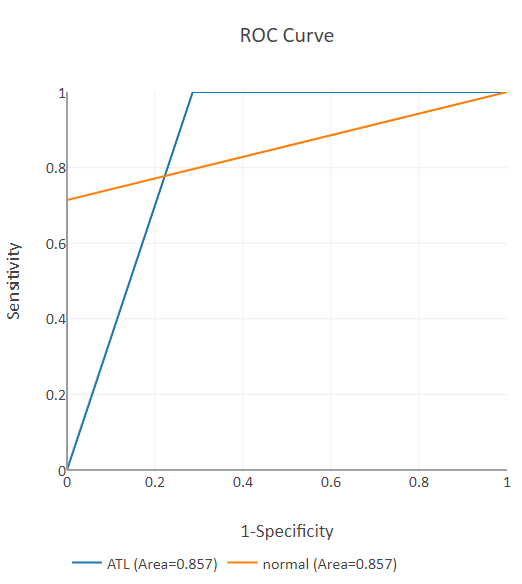
\includegraphics[scale=0.45]{leukemia_gse14317_ROC.PNG}
    \caption{Curva ROC obtenida para el fichero de datos leukemia\_gse14317.csv.}
    \label{fig:5}
\end{figure}



La interpretación gráfica que se hace de la curva ROC no permite comparar diferentes curvas, especialmente en determinados casos en los que el gráfico presenta intervalos con una curva por encima de otra e intervalos en los que esto sucede al revés. La solución que se propone es utilizar el área bajo la curva ROC como un indicador cuantitativo del acierto del modelo. La definición de la curva ROC implica un aumento del área bajo la curva cuanto mayor sea la tasa de acierto sobre la tasa de error, el área bajo la curva ROC para un modelo con una clasificación perfecta es de una unidad, mientras que el área bajo la curva ROC para un modelo que clasifica de forma incorrecta todos los registros es de cero.

\bigbreak

La Figura \ref{fig:5} representa la curva ROC obtenida para un modelo de clasificación binaria. La disposición gráfica de ambas curvas indica que el modelo presenta una notable capacidad discriminatoria entre clases. El área bajo la curva ROC de $0.857$, también indica que el modelo tiene una muy buena tasa de acierto sobre error.

\bigbreak

Existen diferentes métodos para calcular el área bajo la curva, en la sección de experimentación se ha utilizado la regla del trapecio para el calculo de la integral definida entre cero y uno. El método del trapecio consiste en el calculo de los trapecios que forman cada par de puntos consecutivos con la curva. En la ecuación \ref{eq:trapecio} se define el área bajo la curva a partir de la regla del trapecio.

\bigbreak

\begin{equation}
    AUC = \int_{a}^{b} f(x) \,dx = \sum_{k=1}^{N} \frac{f(x_{k-1})+f(x_{k})}{2} \cdot \frac{b-a}{N}
    \label{eq:trapecio}
\end{equation}

\bigbreak

La curva ROC no esta definida para su aplicación en modelos de clasificación multi etiqueta, en estos casos una alternativa es el calculo de una curva ROC por cada una de las etiquetas. Las diferentes curvas se calculan considerando positiva una de las clases y el resto negativas, esto implica un aumento en la complejidad del gráfico, se pasa de un gráfico en el que se representa una sola curva a un gráfico con una curva por cada clase del modelo.

\clearpage

\subsubsection{Curva PR}

La curva PR es un método gráfico que mide el rendimiento de un modelo predictivo a partir de los indicadores de precisión y sensibilidad, esto implica que el método es dependiente del balance entre el número de registros de cada clase. El método fue ideado para su aplicación exclusivamente en modelos de clasificación binaria.

\bigbreak

Para representar las medidas de precisión y sensibilidad se emplea el mismo método utilizado para la curva ROC. La idea consiste en establecer una serie de umbrales de aceptación, los diferentes umbrales definen el porcentaje de probabilidad mínimo para considerar positivo un registro. El objetivo es representar el comportamiento que tiene el modelo ante la variación  del umbral de aceptación. La precisión y la sensibilidad son dos métodos que presentan una proporcionalidad inversa, esto implica que al aumentar uno disminuye el otro y viceversa. Al aumentar la sensibilidad, es decir, al reducir el numero de falsos negativos se establece un umbral de aceptación según el cual todos lo registros son positivos, esto provoca que el numero de falsos positivos aumente y por tanto la precisión disminuya.

\bigbreak


La curva PR representa en el eje de ordenadas la precisión y en el eje de abscisas la sensibilidad. La interpretación de al gráfica es algo diferente a la que ofrece la curva ROC. La curva ROC presenta una curva que empieza en el punto $(0, 0)$ y termina en el punto $(1, 1)$, cuanto mas se aproxime la curva al punto $(0, 1)$ mejor será el modelo. La curva PR por el contrario ofrece una curva que comienza en el punto $(0, 1)$ y termina en el punto $(1, 0)$. El comportamiento ideal es aquel en el que la curva pase por el punto $(1, 1)$, en este punto la sensibilidad y la precisión alcanzan el valor de una unidad.

\bigbreak

La curva PR presenta la necesidad de obtener una forma cuantitativa de medir como de bueno es el resultado que ofrece la gráfica. El indicador más utilizado para este propósito es el área bajo la curva PR, el área bajo la curva PR establece mejores indicadores cuento mas se aproxime la curva al punto de clasificación perfecta $(0, 1)$. Es una medida ideal para comparar diferentes modelos y establecer que modelo tiene un mejor comportamiento a partir de la sensibilidad y la precisión. El calculo del área bajo la curva se puede hacer a través de varios métodos, uno de los mas populares el el método del trapecio, la ecuación \ref{eq:trapecio} define el calculo del método.

\bigbreak

\begin{figure}[htp]
    \centering
    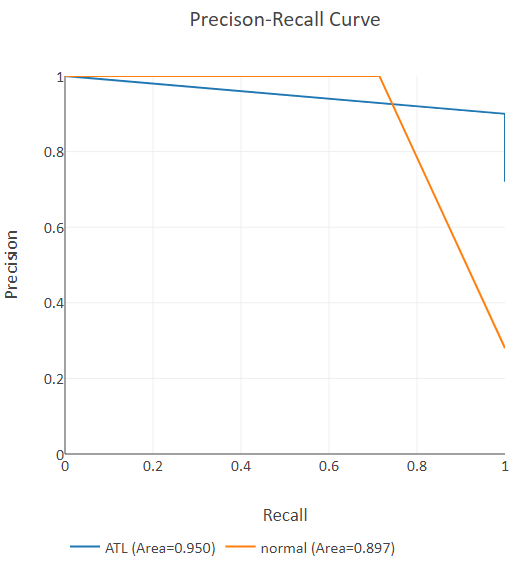
\includegraphics[scale=0.45]{leukemia_gse14317_PR.PNG}
    \caption{Curva PR obtenida para el fichero de datos leukemia\_gse14317.csv.}
    \label{fig:6}
\end{figure}

La definición de la curva PR establece que es método aplicable únicamente a modelos de clasificación binaria, sin embargo, es posible su aplicación a modelos con más de dos clases. La representación que se hace para modelos de clasificación multi etiqueta consiste la generación de una gráfica en la que se incluya una curva por cada una de las clases. En cada curva se considera positiva una de las clases y negativa el resto, la representación que se logra presenta una dificultad mayor a la hora de interpretar los resultados.

\bigbreak

La Figura \ref{fig:6} representa la curva PR obtenida para un modelo de clasificación binaria. La disposición gráfica de ambas curvas indica un buen comportamiento del modelo cuento a tasas de sensibilidad y precisión. El área bajo la curva de $0.950$ para la clase ATL y de $0.897$ para la clase normal indican en general buenas tasas de precisión sobre sensibilidad.

\clearpage